%% Introduction
%%=========================================

\chapter{Introduction}
\label{ch:introduction}
In this chapter we give an introduction to our thesis. First we present the background that our problem relies on. In section \ref{sec:problem_motivation} we present the problem and give a statement about the goals of our thesis. Contributions are summarized in Section \ref{sec:contributions}, and the final section of the chapter presents the structure of the rest of the thesis.

\section{Background}
We find ourselves in the middle of the digital age. The industrial revolution gave us new manufacturing processes at the middle of the seventeenth century, whereas the digital revolution gave us digital electronics, most noticeable the computer \citep{freeman2001time}. With the arrival of high-performance computers and high-speed networks, use of digital technologies increased rapidly. Digital technologies enable information to be created, manipulated, disseminated, relocated, and stored with increasing ease \citep{lee2002state}. This, in combination of increased storage capacities, as well as cheaper storage units, has made digital formats suitable for digital preservation and storage \citep{morris2003evolution}. Due to these benefits, data that used to be store analogue heaps finds new life in digital formats. Photos, audio, video, and books are just a few types of data that are commonly found, or preserved, digitally these days.

\citep{misc-oed-digitization} defines the action or process of digitizing, the task of converting analogue data into digital data, as ``digitization". Google Inc.\footnote{\url{https://www.google.com/intl/en/about/}} and their service Google Books\footnote{\url{https://books.google.com}} is one prime example of mass digitization. Google Books is a service that provides full text of books and magazines online. Other similar projects like Google Books include JSTOR\footnote{\url{https://www.jstor.org}}, which has digitized nearly a thousand journals, dating back to the mid 19th century, and Bokhylla.no\footnote{\url{http://bokhylla.no}} (The Bookshelf). Bokhylla.no is a project initiated by the National Library of Norway. It was launched in 2009 and aims to provide online access to literature published in Norwegian. The service will contain about 250 000 books when it is completed in 2017 \citep{misc-nb-digial-library}. The underlying purposes of these services vary, where Google's primary goal with Google Books is to provide a search and index service \citep{coyle2006mass}, whereas Bookhylla.no provides enhanced reading environments, where the visitor can read entire books from cover to cover. The service also provides full in-text search of the entire library. 

Despite their different use of digitization, they utilize the same types of technologies. While simply scanning the books will suffice to make the literature available online, other technologies are needed to actually index the content. Indexing is the process of capturing the scanned text and converting it into editable and searchable data. To capture textual data, a technology called Optical Character Recognition, or OCR for short, is used. OCR has many applications, and is in use in many areas today. Book scanning, number plate recognition, handling of checks, passports, as well as assistive technologies for blind and visually impaired users are just some areas which uses OCR today \citep{mori1999optical, kurzweil2000reading}.

%%=========================================

\section{Problem and Motivation}
\label{sec:problem_motivation}
OCR is, in a broad sense, a branch of artificial intelligence, and a research branch in pattern recognition and computer vision \citep{mori1999optical}. It was first believed that it would be easy to develop an OCR, and researchers estimated that an accurate reading machine would be introduced in the 1950s. During the 1950s and the early 1960s researchers were still struggling with an ideal OCR model. Their research has since laid the foundation for modern research in the field \citep{mori1992historical}.

We have come a long way since the 1950s, and \citep{ye2015text} states:

\begin{quote}
    While many researchers view optical character recognition (OCR) as a solved problem, text detection and recognition in imagery possess many of the same hurdles as computer vision and pattern recognition problems driven by lower quality or degraded data.
\end{quote}

Under optimal conditions, certain OCR systems can perform very well. OCR has reached great results in clean and well-formatted documents, in some cases achieving up to 99\% recognition rates. In cases where the documents are not clean and well-formatted, with an OCR facing variations of text layouts and fonts, uneven illuminations, and other obstacles, the challenge is much greater. Under these conditions the OCR systems have lower rates of detection and recognition \citep{ye2015text}.

The fact that OCR systems still struggle under sub-optimal conditions indicates that the problem is in fact not solved, and that there is still room for improvements and experimentation with new approaches. One of the area that still have room for improvement is recognizing characters that are damaged or obfuscated. Text can be damaged for a number of reasons, such as pasting of paper, ink spreading, fading, or dirt \citep{bhardwaj2014imaging}. In this thesis we take on a special kind of obfuscated text, and present a new way to recognize it by utilizing their ``signature".

\subsection{Real World Example}
\begin{figure}[ht]
    \centering
    
\includegraphics[width=0.8\textwidth]{fig/chapter1/notch_tweet.png}
    \caption[Print screen of Tweet from notch]{Print screen of Tweet from notch}
    \label{ref:notch_twitter}
\end{figure}

An example of the type of obfuscated text we will attempt to handle in this thesis can be found in a Tweet from Markus ``Notch" Persson. Persson is a Swedish video game programmer and designer, and is most famous for crating the highly acclaimed game Minecraft. He was a inveterate user of Twitter, and used to hint or tease upcoming features of the game. Figure \ref{ref:notch_twitter} contains the Tweet from Persson, which was Tweeted on June 12th 2011.

The image he is referring to in his Tweet can be seen in Figure \ref{fig:notch_imgur}. It is a print screen of what looks like a text editor or IDE\footnote{Integrated Development Environment}. Although image is heavily blurred and cropped, some of the text is still partially visible, like the lower portion of the file names in the tab pane at the top of the image. When this Tweet was posted, one user was able to identify the text in the tabs. He installed the same IDE Persson used, and compared the default font in the program to letters that were partially visible the image. His decoded image can be seen in in Figure \ref{fig:notch_eclipse_decoded}. More than four months later, when version 1.7 of Minecraft was released, it was clear that the decoding was correct as big mushrooms started to appear the game\footnote{The experience orbs were postponed, and introduced in the 1.8 update instead.} \citep{misc-minecraft.172-changelog}.

\begin{figure}[h]
    \centering
    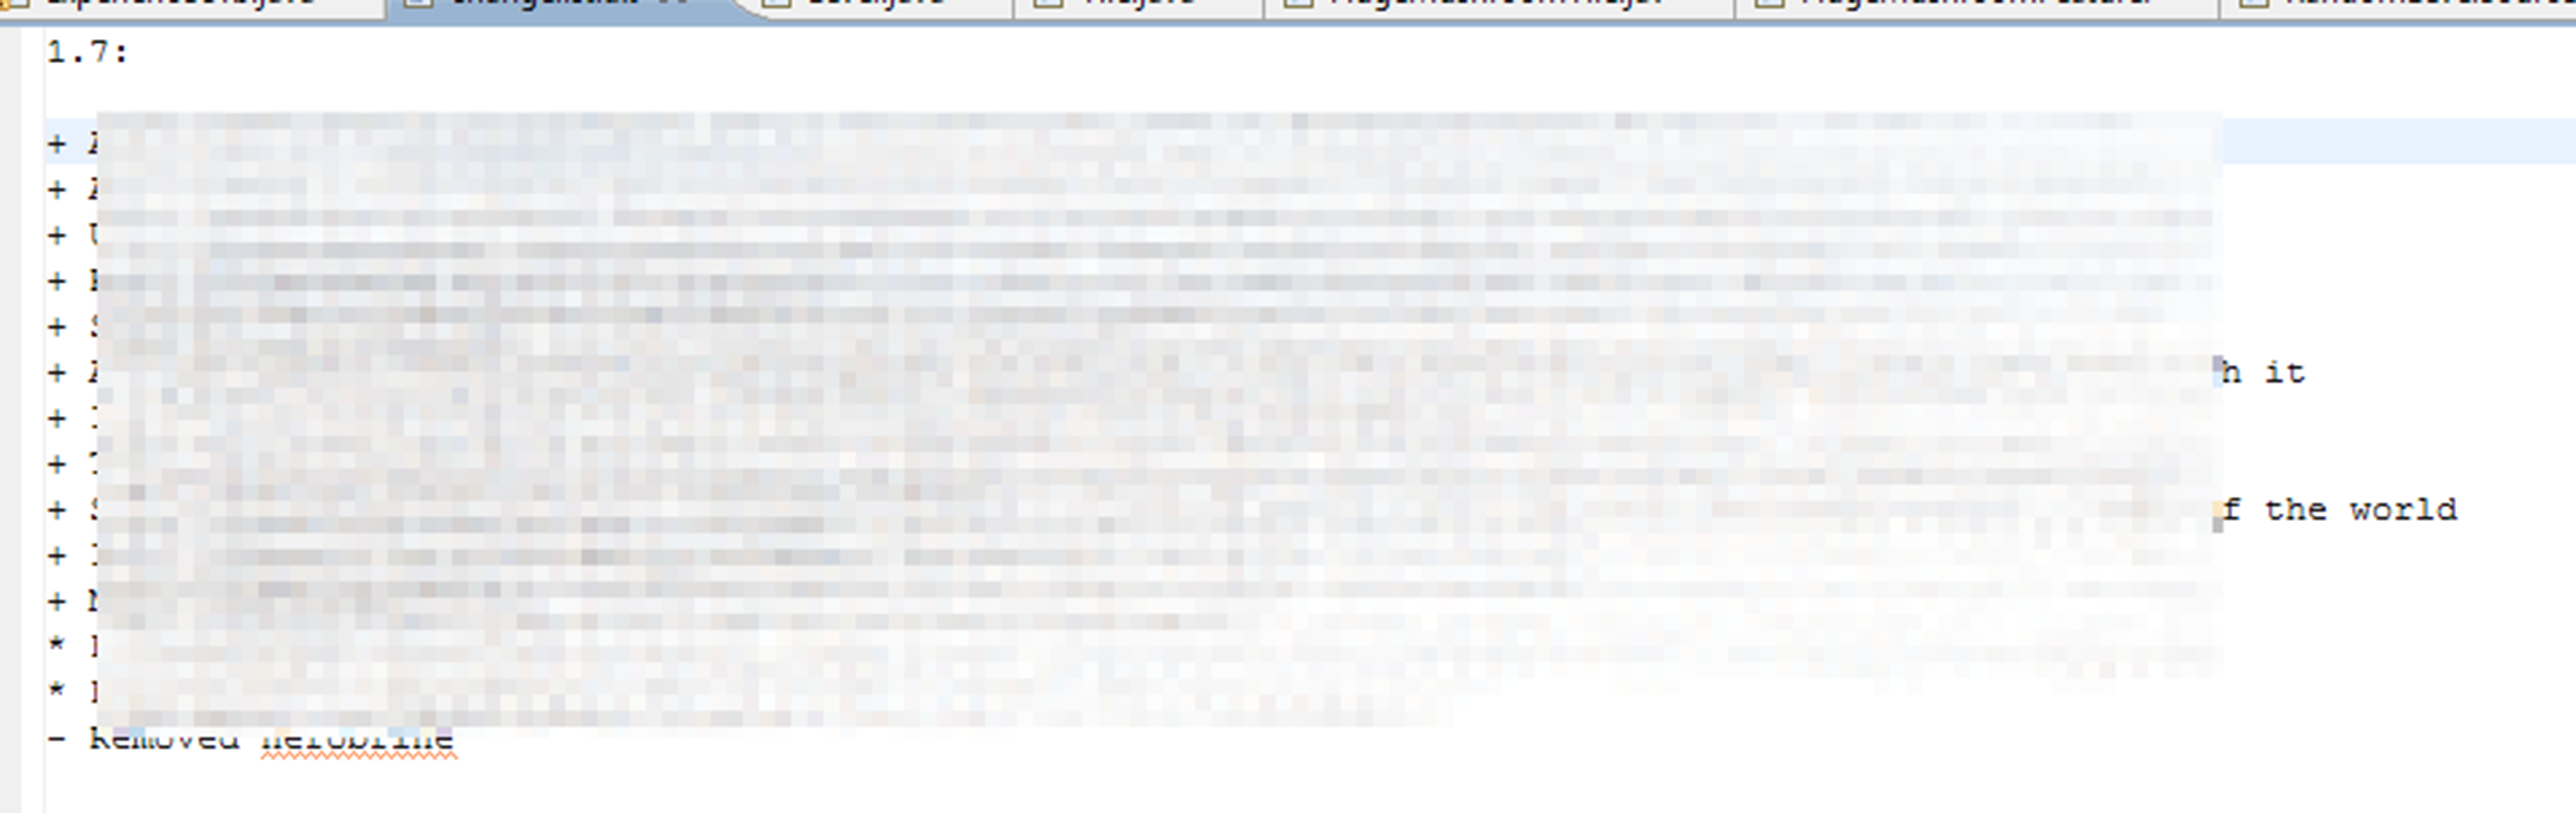
\includegraphics[width=0.8\textwidth]{fig/chapter1/notch_eclipse.png}
    \caption{Blurred image of Minecraft 1.7 changelog from @notch's Tweet}
    \label{fig:notch_imgur}
\end{figure}

\begin{figure}[ht]
    \centering
    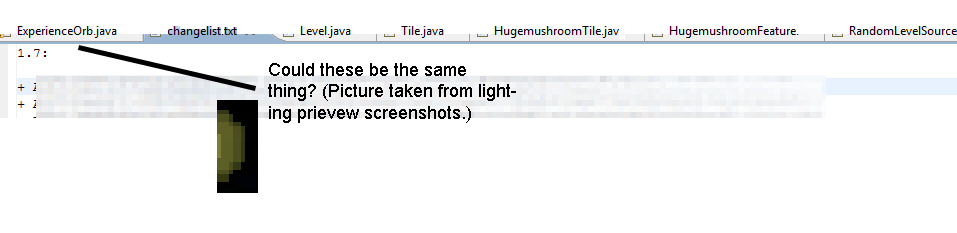
\includegraphics[width=0.8\textwidth]{fig/chapter1/notch_eclipse_decoded.png}
    \caption{Decoding the blurred image from Notch}
    \label{fig:notch_eclipse_decoded}
\end{figure}

\newpage
The decoding that was done to match the letters poses an interesting problem. Can characters and words be recognized given only a very small portion of the glyphs? The decoding in Figure \ref{fig:notch_eclipse_decoded} was done manually by comparing each letter with what was visible, but could such recognition be done automatically? Could such pattern recognition be learned? These questions were used as the basis for this thesis.

%%=========================================

\section{Goals and Research Questions}
\label{sec:goals_and_research_questions}
\begin{figure}[ht]
    \centering
    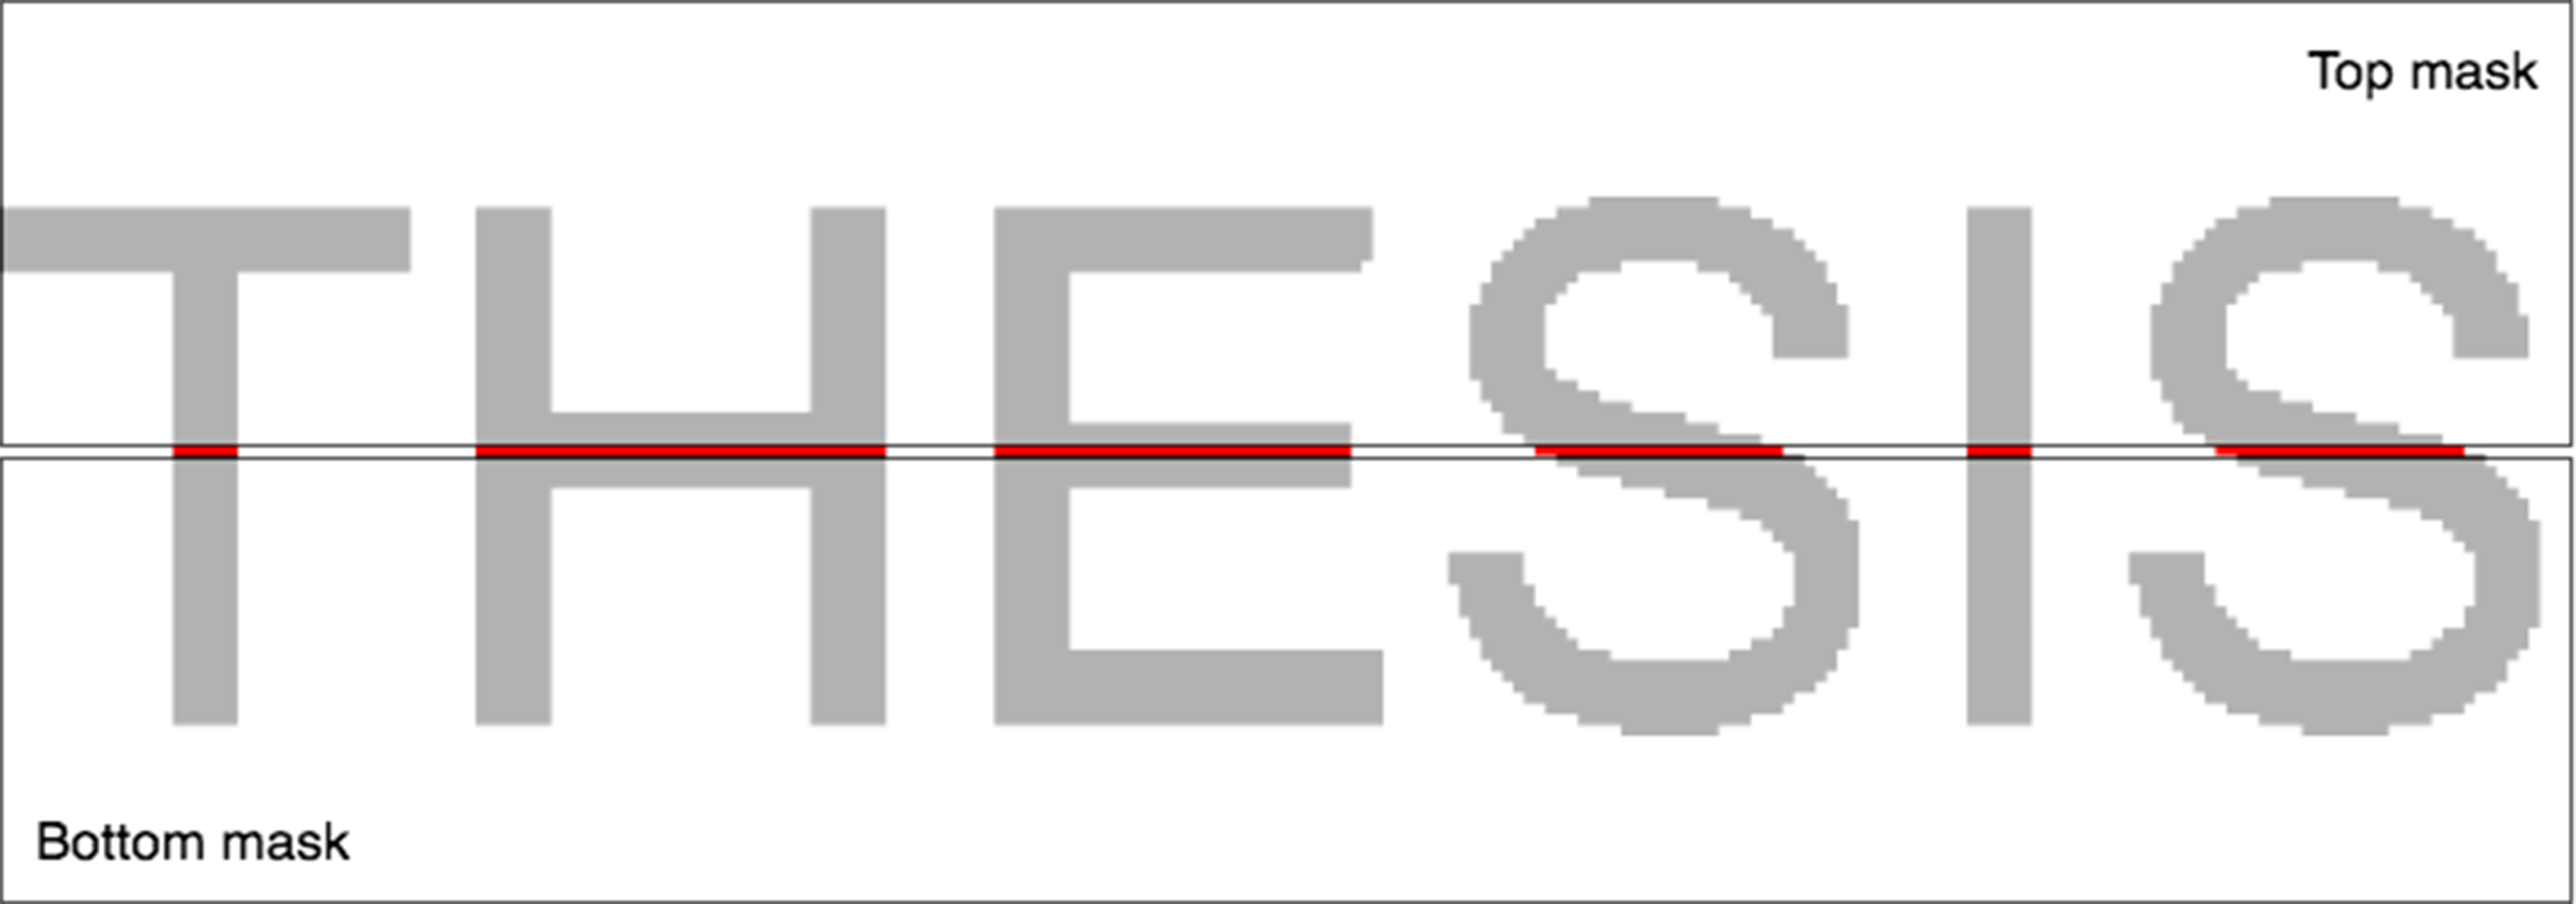
\includegraphics[width=1.\textwidth]{fig/chapter1/signature2.png}
    \caption{Illustration of a word with a signature with a height of one pixel}
    \label{fig:thesis-signature}
\end{figure}

Our goal is to use the ``signature" of letters in a word to recognize it. We can imagine a ``signature" by applying two masks to an image with some written text. These masks spans the total width of the image, and also cover most of the image from the top to bottom, and from the bottom to the top. The only area that is not covered by the masks is a thin line. This line defines the ``signature" for our image and the text written in it. In Figure \ref{fig:thesis-signature} we have a image with the word ``THESIS". The original characters have a height of 50 pixels, and our masks are applied at both the top and bottom of the image. The areas that are covered with masks are translucent, and the only exposed part of the image is a line that has a height of one pixel, here illustrated in red. This line is a ``signature" of the original image. By applying these masks, we omit the data and information that is covered by them, and we do not see the pixels that are translucent in the illustration.

With an approach like the one we present, there are many interesting question that can be raised about a potential system for such problems. While our overarching research goal is to find out if such an approach works at all, there are many ways to explore further on how settings, configurations, and conditions influences the system.

Trying to make the research done in this thesis as valuable as possible, we have focused our research questions on areas that are hopefully are most relevant for further research. Instead of focusing on narrow and niche questions, we have focused on more general and overarching ones. The research questions and their meaning are explained in greater detail in Section \ref{sec:research_questions_and_approach}.

\begin{description}
    \item[Goal]{\textit{Is machine learning able to use signature sequences to recognize words and letters?}}
\end{description}

To expand on the goal stated above, we also have the following research questions that we will attempt to answer during the work on this thesis:

\begin{description}
    \item[Research Question 1]{\textit{Does ambiguity in character signature sequences impact recognition rates?}}
    \item[Research Question 2]{\textit{Can a signature sequence based model handle multiple fonts at the same time?}}
    \item[Research Question 3]{\textit{Is a signature sequence based model unable to handle noise?}}
\end{description}

%%=========================================

\section{Contributions}
\label{sec:contributions}
The contribution of this thesis is mainly the exploration of how to use machine learning and signature sequences to do recognition. The results of the experiments and conclusions done in this thesis may lay the foundation for new way to use machine learning to recognize patterns in data using sequences. Although the ideas presented in this thesis are not new, they may prove that certain problems can be solved using data in different ways. We will also investigate some of the more underlying concepts of the models we develop, and see how they behaved in our problem scenario.

%%=========================================

\section{Thesis Structure}
The remainder of this thesis is structured as follows:

\vspace{0.5cm}\noindent
\begin{minipage}{\linewidth}
    \textbf{{\hyperref[part1]{Part \ref{part1} -- \nameref{part1}}}}
    \begin{itemize}
        \item\textbf{\hyperref[ch:methodology]{Chapter \ref{ch:methodology} -- \nameref{ch:methodology}}} establishes the methodology used throughout the thesis. It explains how the research should be carried out and why we chose the strategies we used.
    \end{itemize}
\end{minipage}

\vspace{0.5cm}\noindent
\begin{minipage}{\linewidth}
    \textbf{{\hyperref[part2]{Part \ref{part2} -- \nameref{part2}}}}
    \begin{itemize}
        \item\textbf{\hyperref[ch:problem]{Chapter \ref{ch:problem} -- \nameref{ch:problem}}} explains the problem in greater detail. It explains the various factors that defines our problem, as well as why it might be a difficult problem to solve. We also look into how we can interpret out problem and how to 
        \item\textbf{\hyperref[ch:background]{Chapter \ref{ch:background} -- \nameref{ch:background}}} introduces some of the concept and ``building blocks" relevant to the proceeding chapter.
        \item\textbf{\hyperref[ch:related_work]{Chapter \ref{ch:related_work} -- \nameref{ch:related_work}}} presents related work done in the area of natural language processing, with a focus on machine translation. We present some of the earlier work as well as establishing the state-of-the-are solutions and work.
    \end{itemize}
\end{minipage}

\vspace{0.5cm}\noindent
\begin{minipage}{\linewidth}
    \textbf{{\hyperref[part3]{Part \ref{part3} -- \nameref{part3}}}}
    \begin{itemize}
        \item\textbf{\hyperref[ch:system_design]{Chapter \ref{ch:system_design} -- \nameref{ch:system_design}}} introduces the system we developed to run our experiments. This includes overall design and general approach, as well as key components.
        \item\textbf{\hyperref[ch:models]{Chapter \ref{ch:models} -- \nameref{ch:models}}} presents the three models we developed as a part of our research on basis of state-of-the-art technologies.
        \item\textbf{\hyperref[ch:experiments]{Chapter \ref{ch:experiments} -- \nameref{ch:experiments}}} establishes how we conducted our experiments, as well how presenting the structure of each experiment and as well as what our goals were. This chapter also presents relevant configuration of the models, and choice of hyper-parameters.
    \end{itemize}
\end{minipage}

\vspace{0.5cm}\noindent
\begin{minipage}{\linewidth}
    \textbf{{\hyperref[part4]{Part \ref{part4} -- \nameref{part4}}}}
    \begin{itemize}
        \item\textbf{\hyperref[ch:results]{Chapter \ref{ch:results} -- \nameref{ch:results}}} presents the results for each experiment explained in the previous chapter. We also discuss the results and evaluate the models.
        \item\textbf{\hyperref[ch:conclusion]{Chapter \ref{ch:conclusion} -- \nameref{ch:conclusion}}} draws the conclusion for our work and present thoughts on possible paths for future work.
    \end{itemize}
\end{minipage}